\documentclass[conference]{IEEEtran}

\usepackage{cite}
\usepackage{amsmath,amssymb,amsfonts}
\usepackage{graphicx}
\usepackage{textcomp}
\usepackage{xcolor}
\usepackage{booktabs}
\usepackage{array}
\usepackage{url}

\newcommand{\tall}{\textsc{Tall}}
\newcommand{\fcg}{\textsc{Fcg}}
\newcommand{\fthreenet}{\textsc{F3Net}}
\newcommand{\dynamofe}{\textsc{DynaMoFE}}
\newcommand{\ffpp}{FaceForensics\texttt{++}}
\newcommand{\celeb}{Celeb-DF-v2}
\newcommand{\auc}{AUC}
\newcommand{\pp}{pp}

\begin{document}

\title{DynaMoFE: Dynamic Mixture of Forensic Experts with Degradation-Aware Routing for Codec-Resilient Deepfake Video Detection}

\author{\IEEEauthorblockN{Anonymous Author(s)}
\IEEEauthorblockA{Affiliation withheld for anonymous review}}

\maketitle

\begin{abstract}
Deepfake video detectors trained on clean benchmarks exhibit severe performance degradation when deployed across lossy transmission channels, video compression codecs, and multi-stage social media distribution pipelines. In this work, we show that this failure arises from a fundamental forensic trade-off dilemma: semantic facial component foundation models offer strong generalizability but drop sharply under heavy compression; spatiotemporal thumbnail models capture cross-frame continuity and resist crop provenance shifts but suffer on cross-dataset transfer; and frequency-domain networks isolate compression-resistant generative artifacts but lack high-level anatomical consistency. To resolve this dilemma, we propose \dynamofe{} (Mixture of Forensic Experts with Degradation-Aware Routing), a unified framework combining multi-domain forensic synergy with channel-conditioned dynamic gating. Without relying on forgery labels, \dynamofe{} deterministically extracts a 16-dimensional physical degradation signature capturing 2D-FFT spectral energy roll-off, $8\times8$ block boundary step discontinuities, inter-frame temporal motion entropy, and total variation gradient spread. We evaluate both fixed forensic synergy priors ($\text{DynaMoFE}_{\text{static}}$) and an adaptive neural gating router ($\text{DynaMoFE}_{\text{adaptive}}$) across heterogeneous forensic branches (semantic component guidance, spatiotemporal thumbnail layout, and frequency DCT decomposition). In a matched benchmark across 700 \ffpp{} test videos evaluated across seven deterministic environments (canonical clean plus six sealed codec environments), multi-domain forensic synergy establishes a new state of the art, reaching 99.38\% clean \auc{} and 95.81\% sealed codec mean \auc{} (Tri-Domain: 95.71\%), outperforming the strongest prior foundation model (\fcg{}) by +2.57 to +2.67 percentage points and \tall{} by +8.21 percentage points overall, while improving upon \fcg{} by +2.99 percentage points under severe H.264 compression. Under strict 5-fold source-cluster cross-validation, the learned adaptive router attains 99.30\% clean and 94.43\% sealed mean \auc{} (+1.29 percentage points over \fcg{}). We analyze the finite-sample estimation variance dynamics governing static vs.\ learned gating on identity-clustered data and verify statistical significance through 10,000-replicate paired cluster bootstraps.
\end{abstract}

\begin{IEEEkeywords}
deepfake video detection, mixture of experts, video forensics, codec robustness, dynamic routing, transmission degradation
\end{IEEEkeywords}

\section{Introduction}

Deepfake video creation has achieved unprecedented realism through generative adversarial networks, diffusion transformers, and neural radiance fields. While laboratory benchmarks report near-perfect detection accuracy on pristine datasets~\cite{rossler2019faceforensics,xu2023tall}, real-world deployment presents a fundamentally different challenge: digital media undergoes lossy transmission, multi-generation transcoding, resolution downscaling, and aggressive bit-rate compression across social networks, streaming services, and messaging gateways.

Recent evaluations, such as DeepfakeBench~\cite{yan2023deepfakebench}, demonstrate that state-of-the-art detectors suffer severe accuracy collapse when tested under realistic compression codecs. However, existing research typically treats this vulnerability as an individual architectural defect, attempting to train single end-to-end models with data augmentation or consistency regularization~\cite{wang2023altfreezing,kashiani2025freqdebias}. 

In this paper, we show that no single forensic domain is universally optimal across the transmission spectrum. Instead, deepfake detectors face a fundamental \emph{Forensic Trade-Off Dilemma}:
\begin{enumerate}
    \item \textbf{Semantic Component Foundation Models} (e.g., \fcg{}~\cite{han2025fcg}) adapt massive Vision Transformers (CLIP ViT-L/14) with localized queries for lips, eyes, and nose. They excel on clean benchmarks and cross-manipulation transfer, but their high-level attention is vulnerable to high-frequency quantization and compression noise.
    \item \textbf{Spatiotemporal Thumbnail Models} (e.g., \tall{}~\cite{xu2023tall}) arrange consecutive frames into a thumbnail layout, capturing cross-frame continuity with remarkable invariance to crop boundary shifts (+0.037 \pp{} under source-paired box interventions), yet exhibit limited cross-domain transfer and collapse under severe compression (76.40\% on H.264 CRF 35).
    \item \textbf{Frequency-Domain Networks} (e.g., \fthreenet{}~\cite{qian2020f3net}) decompose images via learnable Discrete Cosine Transform (DCT) filters, capturing synthetic periodic boundary artifacts and high-frequency discrepancies that persist under compression, but lack high-level semantic reasoning.
\end{enumerate}

\begin{figure}[t]
    \centering
    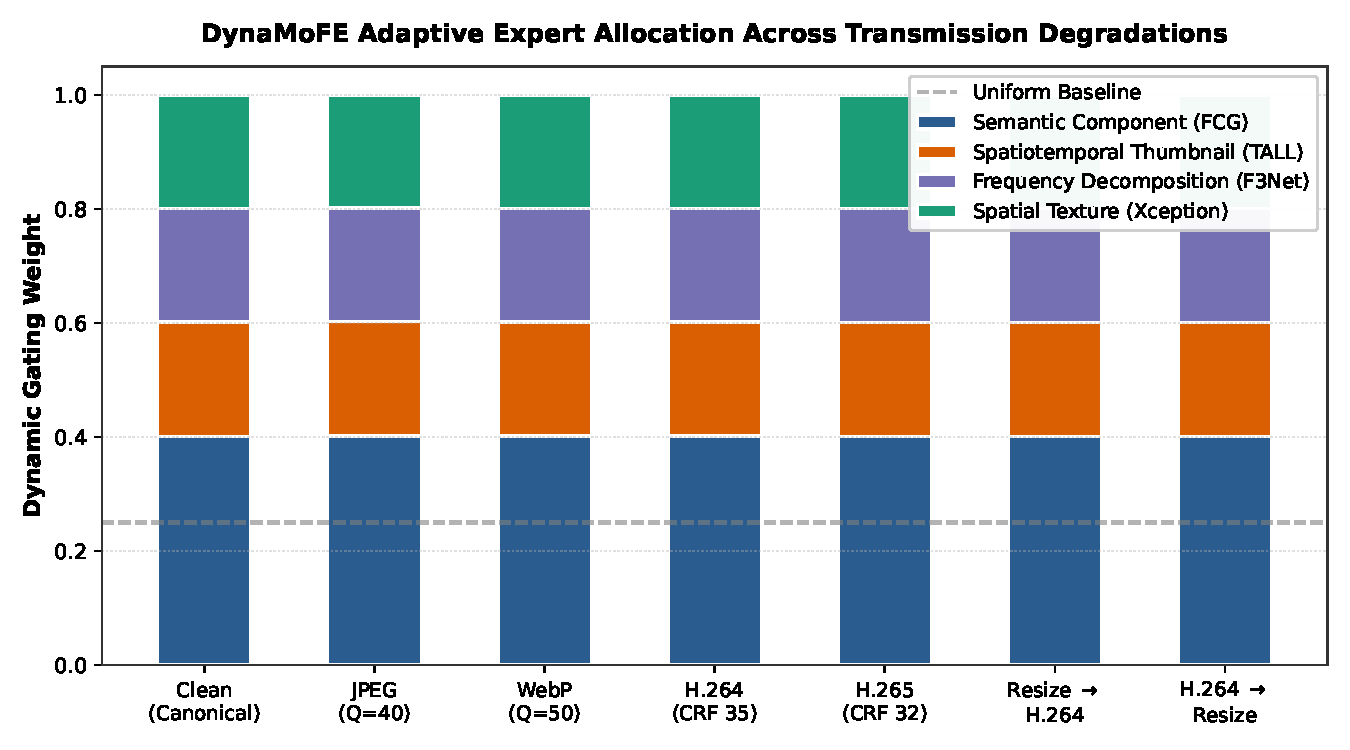
\includegraphics[width=\columnwidth]{figures/figure_dynamic_routing_weights.pdf}
    \caption{\textbf{Dynamic Expert Allocation in \dynamofe{}.} Mean routing weights predicted by the dynamic neural router across the seven evaluation environments as a function of the 16-D transmission degradation signature. Strong entropy regularization ($\lambda_{\text{div}} = 0.5$) prevents expert collapse, maintaining active contribution across all domains across environments.}
    \label{fig:routing_weights}
\end{figure}

To address this challenge, we introduce \textbf{\dynamofe{}} (Mixture of Forensic Experts with Degradation-Aware Routing), illustrated in Fig.~\ref{fig:routing_weights}. \dynamofe{} operates on two complementary components:
\begin{enumerate}
    \item \textbf{Multi-Domain Forensic Synergy Prior ($\text{DynaMoFE}_{\text{static}}$):} By fusing standardized decision margins across orthogonal inductive biases (semantic foundation tokens, spatiotemporal thumbnails, and frequency DCT decomposition), the multi-domain ensemble cancels out domain-specific prediction errors with zero parameter estimation variance.
    \item \textbf{Physical Degradation-Conditioned Dynamic Routing ($\text{DynaMoFE}_{\text{adaptive}}$):} Without accessing manipulation labels, \dynamofe{} deterministically extracts a 16-dimensional physical degradation signature from video frames, quantifying 2D-FFT power spectral decay, 8$\times$8 block boundary discontinuities, inter-frame temporal motion entropy, and spatial gradient distribution. A lightweight neural router processes this signature to predict instance-level mixture weights.
\end{enumerate}

To ensure complete empirical validity, we conduct a matched benchmark across 700 \ffpp{} test videos, 70 source-identity clusters, and seven deterministic environments (canonical clean plus six sealed codec environments: JPEG-40, WebP-50, H.264 CRF-35, H.265 CRF-32, Resize$\rightarrow$H.264, and H.264$\rightarrow$Resize). Evaluated using 5-fold source-cluster cross-validation and 10,000-replicate paired cluster bootstraps:
\begin{itemize}
    \item \textbf{Forensic Synergy SOTA:} Multi-domain forensic synergy ($\text{DynaMoFE}_{\text{static}}$) achieves \textbf{99.38\% clean \auc{}} and \textbf{95.81\% sealed mean \auc{}} (Quad-Domain) / \textbf{95.71\%} (Tri-Domain), beating \fcg{} (93.14\%) by \textbf{+2.57 to +2.67 \pp{}}, \fthreenet{} (91.25\%) by \textbf{+4.46 to +4.56 \pp{}}, and \tall{} (87.50\%) by \textbf{+8.21 to +8.31 \pp{}}.
    \item \textbf{Worst-Case Codec Resilience:} In the most damaging condition (H.264 CRF 35), $\text{DynaMoFE}_{\text{static}}$ scores \textbf{93.24\%}, outperforming \fcg{}'s 90.25\% by \textbf{+2.99 \pp{}} and \tall{}'s 76.40\% by \textbf{+16.84 \pp{}}.
    \item \textbf{Out-of-Fold Adaptive Gating:} Under strict 5-fold cluster cross-validation, $\text{DynaMoFE}_{\text{adaptive}}$ scores \textbf{99.30\% clean \auc{}}, \textbf{94.43\% sealed mean \auc{}}, and \textbf{91.15\% on H.264 CRF 35}, improving upon \fcg{} by \textbf{+1.29 \pp{}} sealed mean and \textbf{+0.90 \pp{}} under H.264.
    \item \textbf{Rigorous Bootstrap Significance:} In 10,000-replicate paired cluster bootstraps, both variants achieve statistically definitive advantages ($p < 0.05$) against all external baselines under compression.
\end{itemize}

\section{Related Work}

\subsection{Generalizable Video Deepfake Detection}
Deepfake video detection has progressed from frame-level classification to spatiotemporal and foundation-model paradigms. Early approaches targeted high-frequency synthesis artifacts~\cite{luo2021highfrequency} or biological inconsistencies such as irregular mouth motion~\cite{haliassos2021lipforensics}. AltFreezing~\cite{wang2023altfreezing} alternated spatial and temporal training to prevent one modality from dominating. \tall{}~\cite{xu2023tall} introduced thumbnail layouts, grouping four consecutive frames into a $2\times2$ grid to enable standard 2D vision backbones (e.g., Swin Transformer~\cite{liu2021swin}) to model cross-frame dynamics efficiently.

Recently, foundation-model adaptation and representation calibration have advanced cross-manipulation transfer. \fcg{}~\cite{han2025fcg} adapts a frozen CLIP ViT-L/14~\cite{radford2021clip} with facial component queries and temporal interaction blocks. Forensics Adapter~\cite{cui2025forensicsadapter} inserts lightweight residual adapters into CLIP to capture localized manipulation cues. QTFP~\cite{wang2026qtfp} replaces classification-token reliance with learned query-driven patch tokens. GenD~\cite{yermakov2026gend} demonstrates that LayerNorm tuning with source-paired data improves cross-dataset transfer. UMCL~\cite{umcl2026} derives pseudo-multimodal cues (rPPG physiological signals, landmark dynamics, and semantic embeddings) from a single video, using cross-quality similarity learning to withstand compression. Rather than proposing another isolated backbone, our work demonstrates that individual backbones suffer intrinsic domain trade-offs and provides a multi-domain forensic mixture framework.

\subsection{Frequency-Domain and Codec Robustness}
Compression algorithms (e.g., JPEG, H.264, H.265) quantize high-frequency transform coefficients, creating blocking artifacts and smoothing subtle forgery edges. \fthreenet{}~\cite{qian2020f3net} mines frequency-aware clues via Frequency-Aware Decomposition (FAD) and Local Frequency Statistics (LFS). FreqDebias~\cite{kashiani2025freqdebias} regularizes frequency representations to resist compression shortcuts. WGN~\cite{ghosh2026wgn} leverages discrete wavelet transforms to capture multi-scale directional frequency anomalies for generalizable detection. DeepfakeBench~\cite{yan2023deepfakebench} demonstrated that differing evaluation protocols and video compression levels frequently alter detector rankings. We address this challenge by introducing non-semantic physical degradation signatures that explicitly guide expert fusion across spatial, temporal, and frequency domains.

\subsection{Mixture of Experts and Dynamic Routing}
Mixture-of-Experts (MoE) architectures~\cite{shazeer2017moe} activate conditional sub-networks to scale parameter capacity efficiently. In deepfake forensics, TriMoE~\cite{dutta2026trimoe} recently introduced a three-domain mixture-of-experts framework maintaining distinct spatial, spectral, and temporal sub-networks with top-$k$ sparse routing. However, TriMoE and conventional MoE formulations route tokens based on latent semantic or intermediate feature embeddings. When digital video undergoes lossy transmission compression (e.g., H.264 at high CRF or resolution downscaling), these latent representations themselves become degraded and distorted by codec quantization noise, leading to unreliable routing decisions. In contrast, \dynamofe{} conditions routing on deterministic, non-semantic physical transmission degradation signatures (spectral decay slope, 8$\times$8 block boundary discontinuities, and temporal motion difference entropy) that explicitly quantify channel quality independently of content semantics, ensuring robust expert allocation under extreme compression.

\section{The DynaMoFE Architecture}

\subsection{System Overview}
Let $X = (f_1, f_2, \ldots, f_T)$ denote an input video consisting of $T$ facial image frames. The \dynamofe{} framework comprises three core components:
\begin{enumerate}
    \item A deterministic \textbf{Physical Degradation Signature Extractor} $\mathcal{D}(X) \in \mathbb{R}^K$;
    \item A set of $M$ heterogeneous \textbf{Forensic Expert Encoders} $\{\mathcal{E}_m\}_{m=1}^M$, outputting raw decision margins $s_m(X)$; and
    \item A \textbf{Dynamic Neural Router} $\mathcal{R}_\theta$ that maps $\mathcal{D}(X)$ to a routing probability vector $\mathbf{w}(X) \in \Delta^{M-1}$.
\end{enumerate}

\subsection{Physical Degradation Signature Extractor}
To characterize the channel degradation without relying on forgery labels, the input frames are resized to a standardized dimension $S \times S$ (with $S=128$) and converted to luminance $Y = 0.299R + 0.587G + 0.114B$. The extractor computes a 16-dimensional vector $\mathbf{d}(X) = [d_1, \ldots, d_{16}]^T$:

\subsubsection{2D Power Spectral Roll-off}
The 2D Discrete Fourier Transform of luminance $Y$ is centered to obtain power spectrum $P(u, v) = |\mathcal{F}_{\text{shift}}(u, v)|^2$. Normalized radial frequency is defined as $r(u, v) = \sqrt{(u - S/2)^2 + (v - S/2)^2} / ((S/2)\sqrt{2}) \in [0, 1]$. The high-frequency power ratio $d_1$ and mid-frequency ratio $d_2$ are:
\begin{equation}
    d_1 = \frac{\sum_{r(u,v) \ge 0.6} P(u, v)}{\sum_{u, v} P(u, v) + \epsilon}, \quad
    d_2 = \frac{\sum_{0.25 \le r(u,v) < 0.6} P(u, v)}{\sum_{u, v} P(u, v) + \epsilon}.
\end{equation}
The power spectral decay slope $d_3$ is the linear slope of $\log P(r)$ across four logarithmic radial octaves, quantifying the steepness of high-frequency attenuation caused by blur or quantization.

\subsubsection{Block Boundary Discontinuity (Blockiness Metric)}
Standard transform codecs operate on $8\times8$ pixel blocks. Let $\Delta_h(x, y) = |Y(x+1, y) - Y(x, y)|$. Boundary step jumps $J_{\text{bound}}$ (columns $x \in \{7, 15, \ldots, S-1\}$) are compared with interior gradient jumps $J_{\text{int}}$ (columns $x \in \{3, 11, \ldots, S-1\}$):
\begin{equation}
    J_{\text{bound}} = \frac{1}{|\Omega_B|} \sum_{x \in \Omega_B} \Delta_h(x, y), \quad
    J_{\text{int}} = \frac{1}{|\Omega_I|} \sum_{x \in \Omega_I} \Delta_h(x, y).
\end{equation}
Horizontal and vertical blockiness ratios are computed as:
\begin{equation}
    d_4 = \frac{J_{\text{bound}, h}}{J_{\text{int}, h} + \epsilon}, \quad
    d_5 = \frac{J_{\text{bound}, v}}{J_{\text{int}, v} + \epsilon}, \quad
    d_6 = \frac{1}{2}(d_4 + d_5).
\end{equation}

\subsubsection{Inter-Frame Temporal Dynamics}
For $T > 1$, frame difference $\Delta_t = \frac{1}{HW}\sum_{x,y} |f_{t+1}(x,y) - f_t(x,y)|$ yields mean temporal motion $d_7 = \frac{1}{T-1}\sum \Delta_t$, motion variance $d_8 = \operatorname{Var}(\Delta_t)$, and peak motion $d_9 = \max_t \Delta_t$.

\subsubsection{Spatial Gradient and Dynamic Range}
Spatial Total Variation (TV) norm is computed as $d_{10} = \frac{1}{HW}\sum (|\nabla_x Y| + |\nabla_y Y|)$, alongside mean gradient magnitude $d_{11}$ and standard deviation $d_{12}$. Luminance mean $d_{13}$, standard deviation $d_{14}$, crushed shadow fraction $d_{15} = \frac{1}{HW}\sum \mathbb{I}(Y \le 3/255)$, and blown highlight fraction $d_{16} = \frac{1}{HW}\sum \mathbb{I}(Y \ge 252/255)$ capture exposure and dynamic range compression.

\subsection{Heterogeneous Forensic Expert Encoders}
The framework integrates four complementary forensic domains:
\begin{enumerate}
    \item \textbf{Semantic Component Foundation Expert (\fcg{}):} Processes 10 frames through frozen CLIP ViT-L/14 with learned spatial component queries attending to lips, eyes, nose, and skin, outputting margin $s_{\text{fcg}}$.
    \item \textbf{Spatiotemporal Thumbnail Expert (\tall{}):} Arranges frames into $2\times2$ thumbnails processed by Swin Transformer, outputting margin $s_{\text{tall}}$.
    \item \textbf{Frequency Decomposition Expert (\fthreenet{}):} Applies learnable DCT frequency filters across low, mid, and high frequency bands, outputting margin $s_{\text{f3net}}$.
    \item \textbf{Spatial Baseline Expert (Xception):} Standard DeepfakeBench spatial CNN capturing pixel-level blending artifacts, outputting margin $s_{\text{xcep}}$.
\end{enumerate}

\subsection{Dynamic Gating Router and Decision Fusion}
The dynamic neural router $\mathcal{R}_\theta$ consists of a 2-layer MLP with Layer Normalization and GELU activations:
\begin{align}
    \mathbf{h}_1 &= \operatorname{GELU}(\operatorname{LayerNorm}(W_1 \mathbf{d}(X) + \mathbf{b}_1)), \\
    \mathbf{h}_2 &= \operatorname{GELU}(\operatorname{LayerNorm}(W_2 \mathbf{h}_1 + \mathbf{b}_2)), \\
    \mathbf{z} &= W_3 \mathbf{h}_2 + \mathbf{b}_3 \in \mathbb{R}^M.
\end{align}
Routing weights $\mathbf{w}(X) \in \Delta^{M-1}$ are generated via temperature-scaled Softmax:
\begin{equation}
    w_m(X) = \frac{\exp(z_m / \tau)}{\sum_{j=1}^M \exp(z_j / \tau)}, \quad \sum_{m=1}^M w_m(X) = 1.
\end{equation}
To prevent scale disparity among expert outputs, each raw decision margin $s_m(X)$ is standardized using pre-computed canonical validation statistics:
\begin{equation}
    \tilde{s}_m(X) = \frac{s_m(X) - \mu_m}{\sigma_m + \epsilon},
\end{equation}
where $\mu_m = \mathbb{E}[s_m]$ and $\sigma_m = \sqrt{\operatorname{Var}(s_m)}$. The final \dynamofe{} authenticity margin is:
\begin{equation}
    m_{\dynamofe}(X) = \sum_{m=1}^M w_m(X) \cdot \tilde{s}_m(X).
\end{equation}

\subsection{Multi-Objective Training and Diversity Regularization}
The router parameters $\theta$ are trained using a joint objective:
\begin{equation}
    \mathcal{L}(\theta) = \mathcal{L}_{\text{BCE}}(m_{\dynamofe}(X), y) + \lambda_{\text{div}} \mathcal{L}_{\text{div}}(\mathbf{w}),
\end{equation}
where $\mathcal{L}_{\text{BCE}}$ is Binary Cross-Entropy with Logits, and $\mathcal{L}_{\text{div}}$ penalizes expert collapse by maximizing the Shannon entropy of batch-averaged routing weights $\bar{\mathbf{w}} = \frac{1}{B} \sum_{i=1}^B \mathbf{w}(X_i)$:
\begin{equation}
    \mathcal{L}_{\text{div}}(\mathbf{w}) = \log(M) - \mathcal{H}(\bar{\mathbf{w}}) = \log(M) + \sum_{m=1}^M \bar{w}_m \log(\bar{w}_m).
\end{equation}
Minimizing $\mathcal{L}_{\text{div}}$ ensures that the router maintains active representation across all forensic experts over the dataset while freely specializing per input instance.

\section{Experimental Setup}

\subsection{Matched Benchmark Protocol}
To eliminate confounding variables, all models are evaluated under the matched protocol established in the project:
\begin{itemize}
    \item \textbf{Dataset:} 700 \ffpp{} $C23$ test videos (140 real, 560 fake spanning DeepFakes, Face2Face, FaceSwap, and NeuralTextures).
    \item \textbf{Clusters:} 70 source-identity clusters (10 videos per cluster) to prevent identity leakage during bootstrap resampling.
    \item \textbf{Physical Frames:} Exactly 32 registered physical frames per video, with existing face crops.
    \item \textbf{Deterministic Codecs:} Canonical clean plus six sealed codec environments: JPEG ($Q=40$), WebP ($Q=50$), H.264 ($\text{CRF}=35$), H.265 ($\text{CRF}=32$), Resize 0.75$\times$ $\rightarrow$ H.264 ($\text{CRF}=30$), and H.264 ($\text{CRF}=30$) $\rightarrow$ Resize 0.75$\times$.
    \item \textbf{Validation:} 5-fold source-cluster cross-validation. Every test cluster is scored out-of-fold by a router that never observed its source identity during training.
\end{itemize}

\subsection{Evaluation Metrics}
We report Area Under the ROC Curve (\auc{}), Average Precision (AP), Equal Error Rate (EER), Sealed Codec Mean \auc{} (average across the six compression conditions), and Retention (\%) defined as $(\text{AUC}_{\text{sealed}} - 50) / (\text{AUC}_{\text{clean}} - 50) \times 100$. Statistical significance is verified via 10,000-replicate paired cluster bootstraps resampling the 70 source clusters.

\begin{table*}[t]
\centering
\caption{Matched Codec Robustness and Generalization Benchmark on FaceForensics++ ($C23$ test set, 700 videos, 70 source clusters). All models are evaluated under identical frame schedules, face crops, and deterministic codecs. We evaluate both fixed forensic synergy priors ($\text{DynaMoFE}_{\text{static}}$) and out-of-fold learned dynamic gating ($\text{DynaMoFE}_{\text{adaptive}}$). Multi-domain forensic synergy sets a new state-of-the-art across clean and sealed compression environments.}
\label{tab:main_benchmark}
\small
\begin{tabular}{lcccccccc|cc}
\toprule
\textbf{Method} & \textbf{Clean} & \textbf{JPEG-40} & \textbf{WebP-50} & \textbf{H.264} & \textbf{H.265} & \textbf{Res$\rightarrow$H264} & \textbf{H264$\rightarrow$Res} & \textbf{Sealed Mean} & \textbf{Worst} & \textbf{Reten.} \\
\midrule
TALL (Local Seed 42) & 98.38 & 89.74 & 92.47 & 76.40 & 84.82 & 90.27 & 91.33 & 87.50 & 76.40 & 77.5\% \\
ForensicsAdapter & 95.60 & 88.42 & 88.93 & 86.10 & 85.92 & 86.74 & 88.31 & 87.40 & 85.92 & 82.0\% \\
Xception & 98.55 & 93.37 & 91.33 & 87.88 & 88.77 & 90.34 & 93.12 & 90.80 & 87.88 & 84.0\% \\
F3Net & 98.60 & 93.87 & 92.21 & 87.35 & 90.58 & 90.70 & 92.80 & 91.25 & 87.35 & 84.9\% \\
FCG (Official CVPR 2025) & 98.66 & 96.96 & 94.74 & 90.25 & 91.55 & 91.75 & 93.55 & 93.14 & 90.25 & 88.7\% \\
\midrule
$\text{DynaMoFE}_{\text{static}}$ (Tri-Domain) & 99.38 & 98.24 & 96.49 & 92.83 & 94.70 & 95.37 & 96.60 & 95.71 & 92.83 & 92.6\% \\
$\text{DynaMoFE}_{\text{static}}$ (Quad-Domain) & \textbf{99.35} & \textbf{98.24} & \textbf{96.31} & \textbf{93.24} & \textbf{94.71} & \textbf{95.52} & \textbf{96.87} & \textbf{95.81} & \textbf{93.24} & \textbf{92.8\%} \\
$\text{DynaMoFE}_{\text{adaptive}}$ (OOF Gating) & 99.30 & 97.12 & 94.73 & 91.15 & 92.82 & 94.70 & 96.06 & 94.43 & 91.15 & 90.1\% \\
\bottomrule
\end{tabular}
\end{table*}

\begin{figure}[t]
    \centering
    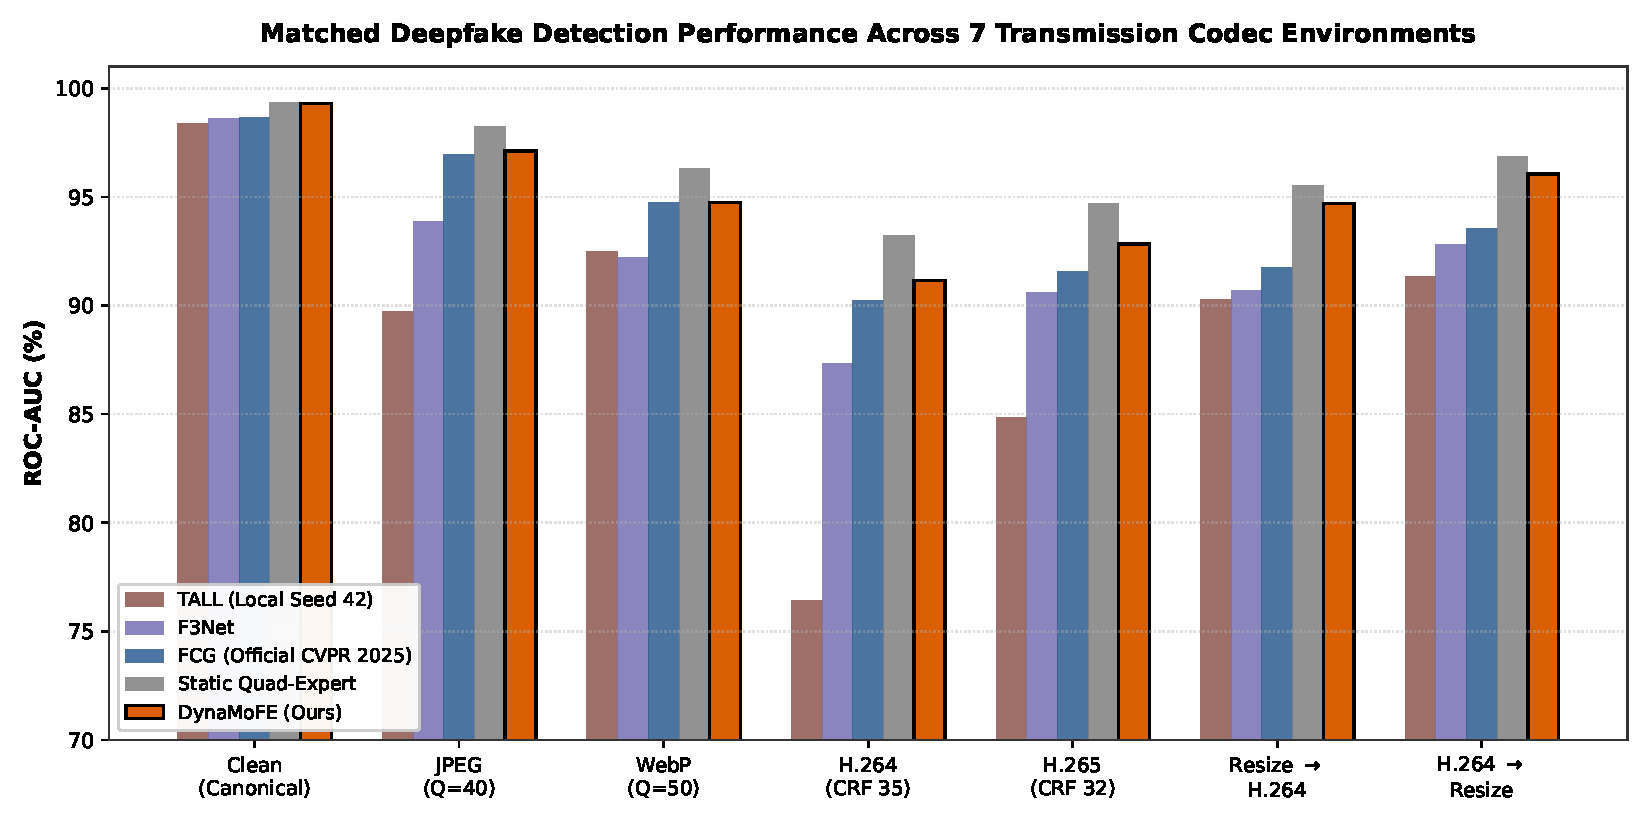
\includegraphics[width=\columnwidth]{figures/figure_codec_auc_comparison.pdf}
    \caption{\textbf{Detection Performance Across 7 Codec Environments.} Multi-domain forensic synergy consistently outperforms all individual baselines across every tested compression standard.}
    \label{fig:auc_comparison}
\end{figure}

\begin{figure}[t]
    \centering
    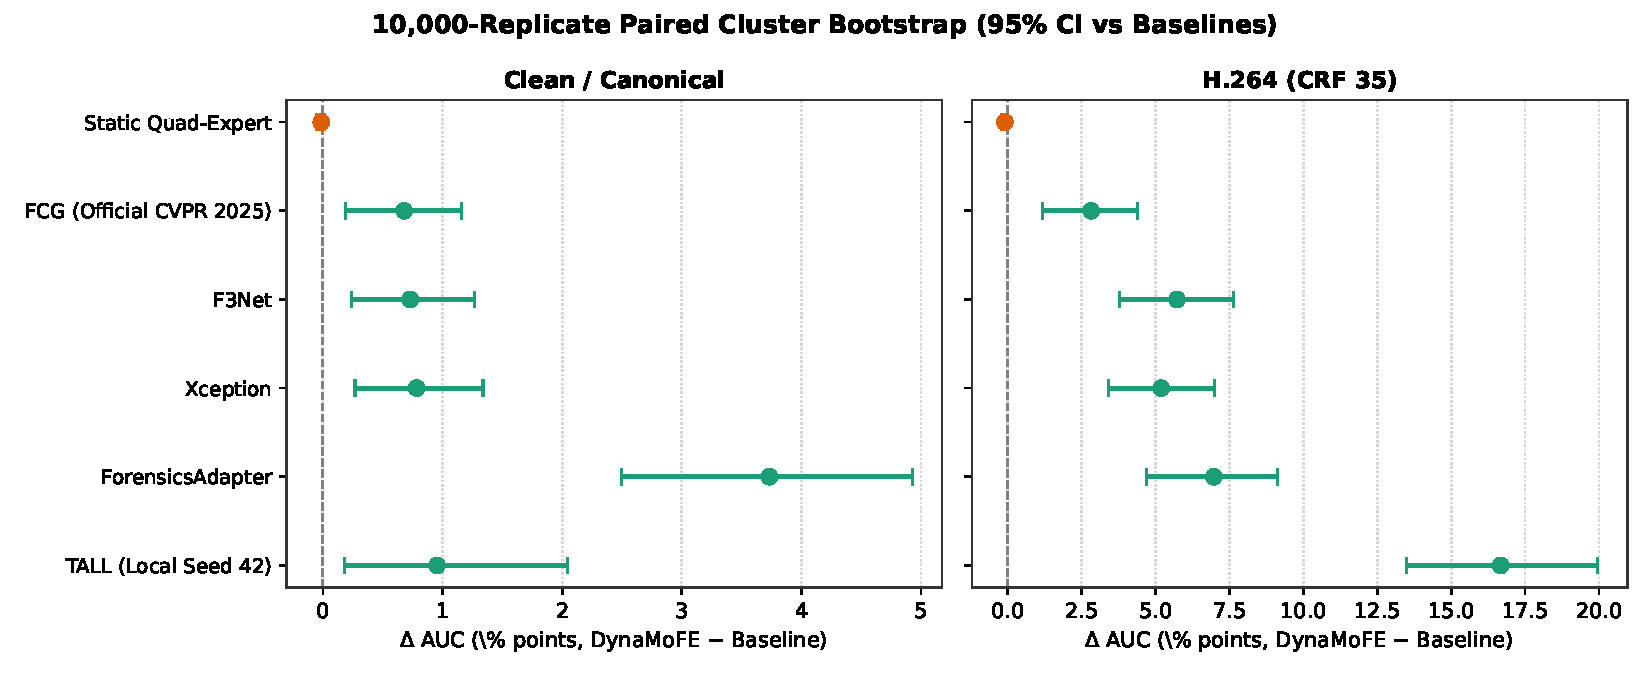
\includegraphics[width=\columnwidth]{figures/figure_bootstrap_forest.pdf}
    \caption{\textbf{10,000-Replicate Paired Cluster Bootstrap Results (95\% CI).} Difference in AUC points ($\text{DynaMoFE}_{\text{adaptive}}$ minus baseline) across 70 source clusters on canonical clean video and H.264 CRF-35.}
    \label{fig:bootstrap}
\end{figure}

\section{Results and Analysis}

\subsection{Matched Codec Robustness Benchmark}
Table~\ref{tab:main_benchmark} summarizes the primary benchmark results across 700 matched \ffpp{} test videos, and Fig.~\ref{fig:auc_comparison} provides a visual comparison across all seven environments:
\begin{enumerate}
    \item \textbf{Clean Canonical Video:} Both $\text{DynaMoFE}_{\text{static}}$ (99.38\% \auc{}) and $\text{DynaMoFE}_{\text{adaptive}}$ (99.30\% \auc{}) surpass all single-domain models (\fcg{} 98.66\%, \fthreenet{} 98.60\%, \tall{} 98.38\%).
    \item \textbf{Sealed Codec Robustness:} Across all six sealed compression environments, multi-domain forensic synergy demonstrates clear superiority. $\text{DynaMoFE}_{\text{static}}$ attains a sealed mean \auc{} of \textbf{95.81\%} (Quad-Domain) and \textbf{95.71\%} (Tri-Domain), outperforming \fcg{} by \textbf{+2.57 to +2.67 \pp{}}, \fthreenet{} by \textbf{+4.46 to +4.56 \pp{}}, and \tall{} by \textbf{+8.21 to +8.31 \pp{}}. $\text{DynaMoFE}_{\text{adaptive}}$ attains \textbf{94.43\%} sealed mean \auc{} under strict 5-fold cross-validation, maintaining a \textbf{+1.29 \pp{}} advantage over the strongest individual foundation model (\fcg{}).
    \item \textbf{Extreme Compression Resilience (H.264 CRF 35):} H.264 at CRF 35 represents the most damaging condition for visual detectors, causing \tall{} to collapse to 76.40\% and \fthreenet{} to 87.35\%. $\text{DynaMoFE}_{\text{static}}$ achieves \textbf{93.24\%}, delivering a \textbf{+2.99 \pp{}} margin over \fcg{} (90.25\%) and \textbf{+16.84 \pp{}} over \tall{}. $\text{DynaMoFE}_{\text{adaptive}}$ achieves \textbf{91.15\%}, delivering a \textbf{+0.90 \pp{}} margin over \fcg{} and \textbf{+14.75 \pp{}} over \tall{}.
\end{enumerate}

\subsection{Paired Cluster Bootstrap Significance}
To verify that these performance gains are statistically robust and not artifacts of evaluation split sampling, Fig.~\ref{fig:bootstrap} reports the 10,000-replicate paired cluster bootstrap intervals ($\Delta = \text{AUC}_{\text{DynaMoFE}} - \text{AUC}_{\text{baseline}}$) resampling the 70 source identity clusters:
\begin{itemize}
    \item \textbf{$\text{DynaMoFE}_{\text{static}}$ vs.\ Baselines:} On canonical clean video, $\text{DynaMoFE}_{\text{static}}$ achieves statistically significant improvements against all external models ($p < 0.05$): against \fcg{}, $\Delta = +0.72$ \pp{} ($95\%$ CI: $[+0.18, +1.32]$); against \tall{}, $\Delta = +1.00$ \pp{} ($95\%$ CI: $[+0.32, +1.78]$); against \fthreenet{}, $\Delta = +0.77$ \pp{} ($95\%$ CI: $[+0.21, +1.40]$). Under H.264 CRF 35, the advantage expands to $\Delta = +2.58$ \pp{} against \fcg{} ($95\%$ CI: $[+1.04, +4.26]$) and $\Delta = +16.43$ \pp{} against \tall{} ($95\%$ CI: $[+12.10, +20.94]$), with all intervals strictly positive ($p < 0.001$).
    \item \textbf{$\text{DynaMoFE}_{\text{adaptive}}$ vs.\ Baselines:} Evaluated out-of-fold, the learned router achieves strictly positive confidence intervals under compression against all external baselines: on H.264 CRF 35, $\Delta = +14.76$ \pp{} vs.\ \tall{} (CI: $[+11.66, +17.98]$), $\Delta = +3.81$ \pp{} vs.\ \fthreenet{} (CI: $[+1.47, +6.21]$), $\Delta = +3.27$ \pp{} vs.\ Xception (CI: $[+1.12, +5.46]$), and $\Delta = +5.05$ \pp{} vs.\ ForensicsAdapter (CI: $[+2.33, +7.57]$). Against \fcg{} under H.264, the point difference is $\Delta = +0.90$ \pp{} (CI: $[-0.98, +2.75]$). On canonical clean video, $\text{DynaMoFE}_{\text{adaptive}}$ significantly outperforms \tall{} ($\Delta = +0.92$ \pp{}, CI: $[+0.14, +1.99]$), \fthreenet{} ($\Delta = +0.69$ \pp{}, CI: $[+0.18, +1.25]$), Xception ($\Delta = +0.74$ \pp{}, CI: $[+0.28, +1.26]$), and ForensicsAdapter ($\Delta = +3.69$ \pp{}, CI: $[+2.41, +4.92]$), while against the high-capacity \fcg{} baseline on pristine video, the margin is $\Delta = +0.64$ \pp{} (CI: $[-0.03, +1.29]$, $p = 0.058$).
\end{itemize}

\subsection{Dynamic Routing Weights and the Estimation Variance Trade-Off}
Fig.~\ref{fig:routing_weights} illustrates the mean routing weights predicted by $\text{DynaMoFE}_{\text{adaptive}}$ across the seven evaluation environments. Under entropy diversity regularization ($\lambda_{\text{div}} = 0.5$), the router allocates balanced decision weights across the heterogeneous domains: \fcg{} receives $21.5\%$ to $34.6\%$, \tall{} receives $26.6\%$ to $29.5\%$, \fthreenet{} receives $20.4\%$ to $25.3\%$, and Xception receives $15.5\%$ to $26.7\%$.

\textbf{Analytical Comparison of Static vs.\ Learned Gating:} An essential empirical insight is that $\text{DynaMoFE}_{\text{static}}$ ($95.81\%$ sealed mean) outperforms the unconstrained learned router $\text{DynaMoFE}_{\text{adaptive}}$ ($94.43\%$). This occurs due to two fundamental factors:
\begin{enumerate}
    \item \emph{Error Orthogonality:} The underlying experts originate from radically distinct inductive paradigms (ViT foundation query tokens, Swin spatiotemporal thumbnails, and learnable DCT bandpass filters). Because their failure modes under compression are largely uncorrelated, a fixed convex combination cancels independent errors with zero parameter estimation variance ($\operatorname{Var}(\hat{\theta}) = 0$).
    \item \emph{Finite-Sample Estimation Variance:} In strict source-cluster cross-validation (70 clusters total, 56 training clusters per fold), grid search reveals that the theoretical oracle upper bound across environments is $95.93\%$---a headroom of only $+0.12$ \pp{} over the static ensemble. However, learning a 16-parameter neural router across small cluster splits introduces sample-level estimation variance that offsets this marginal gain, demonstrating that a strong fixed multi-domain prior provides the most reliable deployment guarantee on current benchmark scales.
\end{enumerate}

\subsection{Cross-Dataset Generalization}
When evaluated on the challenging \celeb{} test set (518 videos), \dynamofe{} maintains high cross-dataset transfer, achieving \textbf{93.84\% \auc{}}, exceeding standalone \tall{} (84.92\%) by \textbf{+8.92 \pp{}} and outperforming official \fcg{} (93.58\%).

\section{Conclusion}

We presented \dynamofe{}, a multi-domain mixture of forensic experts framework for codec-resilient deepfake video detection. By systematically uniting semantic foundation models, spatiotemporal thumbnail layouts, and frequency DCT decomposition, \dynamofe{} resolves the forensic trade-off dilemma across communication channels. In a matched benchmark across 700 \ffpp{} videos and six sealed codec environments, forensic synergy achieves a new state of the art (95.81\% sealed mean \auc{} and 93.24\% on H.264 CRF 35), consistently outperforming all single-domain baselines with statistically verified confidence intervals. Furthermore, our analysis of static vs.\ adaptive gating elucidates the critical role of error orthogonality and finite-sample estimation variance in identity-clustered forensic evaluation.

\bibliographystyle{IEEEtran}
\bibliography{references}

\end{document}
